\section{Introduction to binary tree}
\begin{itemize}
    \item In a binary search tree, the elements have a hierarchical relationship or \emph{parent-child} relationship. These are not linear data structures, linked lists, arrays, stacks, queues are all linear because they do not have a hierarchy. 
    \item Any tree has hierarchical relationships. 
\end{itemize}

\subsection{Examples of binary trees}
\begin{itemize}
    \item A tree can have 0,1 or at most two children.
    \item Each child has 0 or 1 parent. 
    \item The root node is the only node that can have no parents. 
    \item A root can have an empty right tree and an empty left tree. 
    \item The definition of binary trees is recursive, since for instance we can remove node $A$ and be left with two trees by themselves, in this case $B$ would be the root for the left tree, and $C$ would be the root for the right tree. 
        \begin{figure}[H]
            \centering
            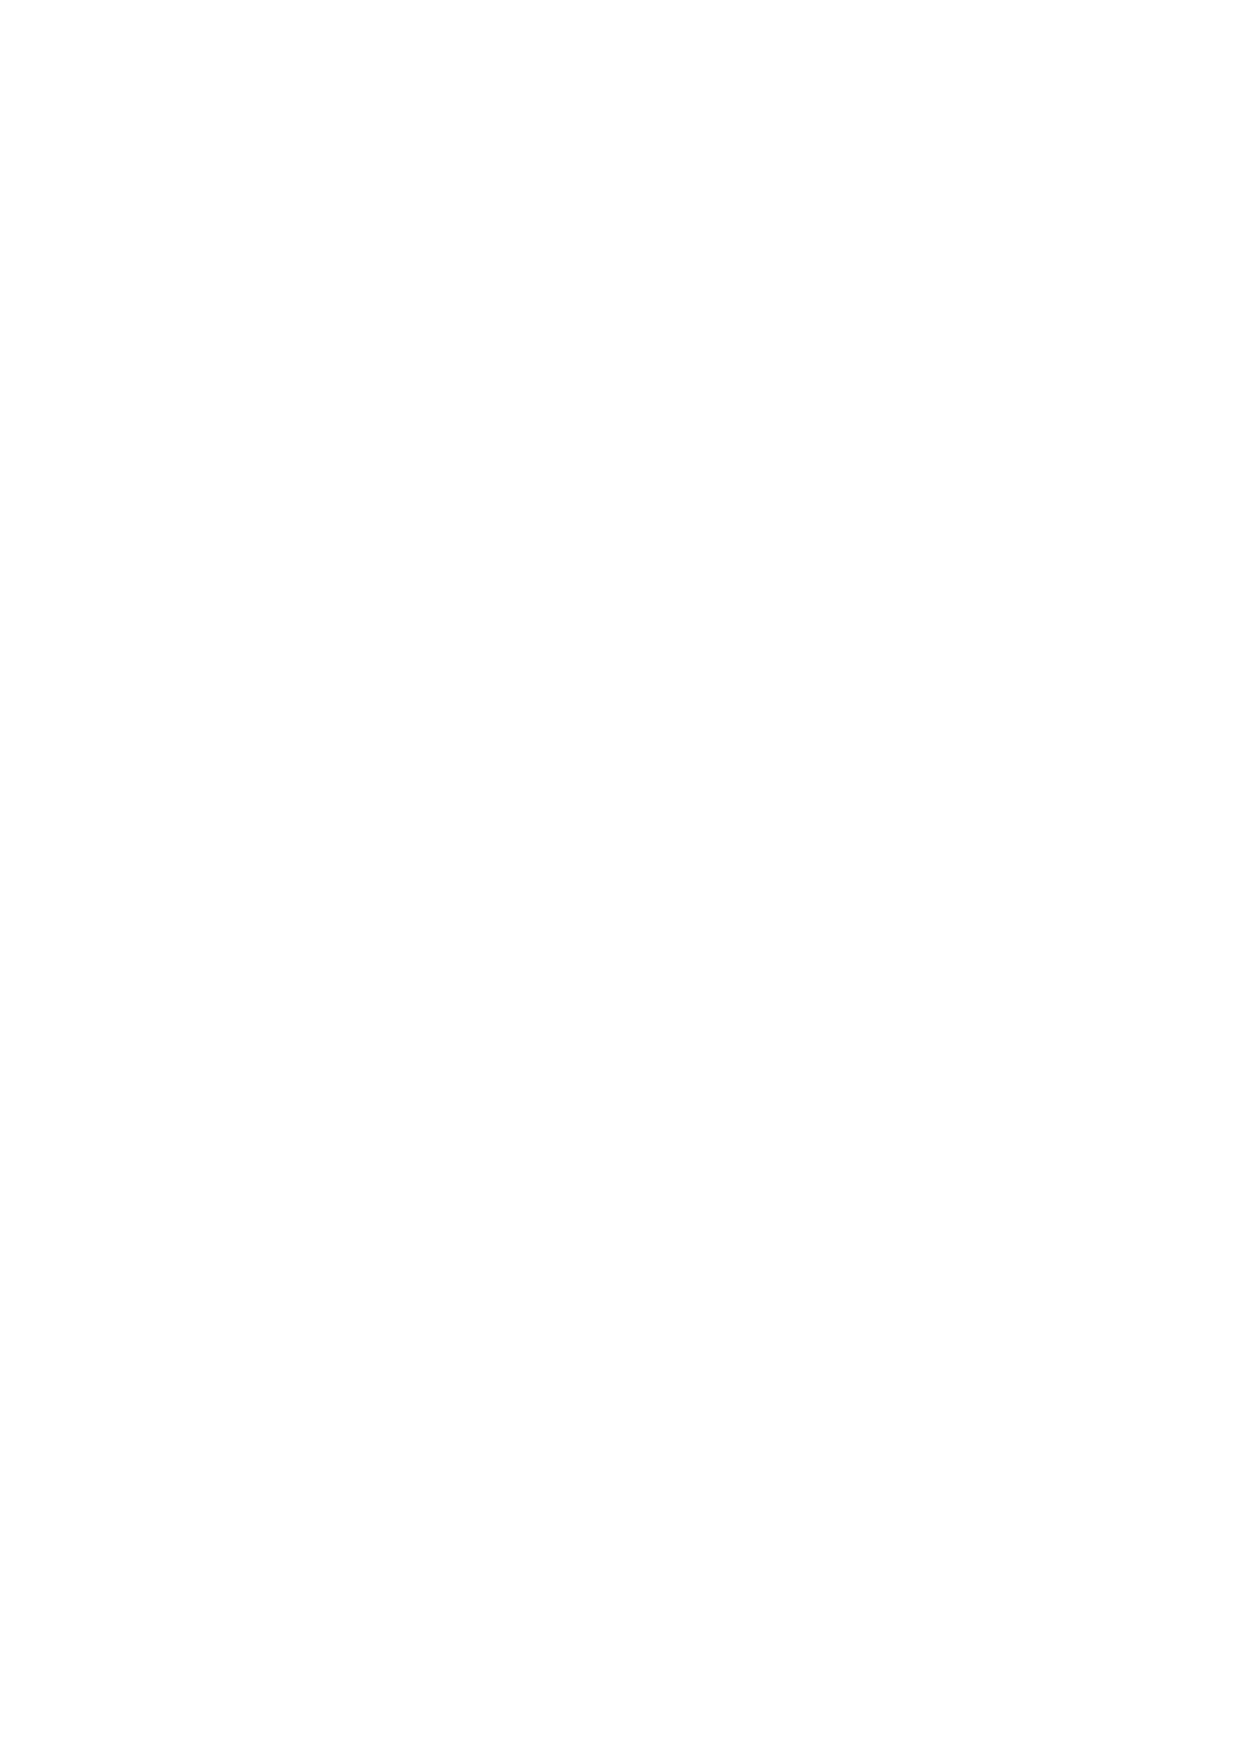
\includegraphics[width=\textwidth]{\figs/binarysearchtreeexample} 
        \end{figure}
\end{itemize}

\subsection{Valid examples and non-valid examples}
\begin{figure}[H]
    \centering
    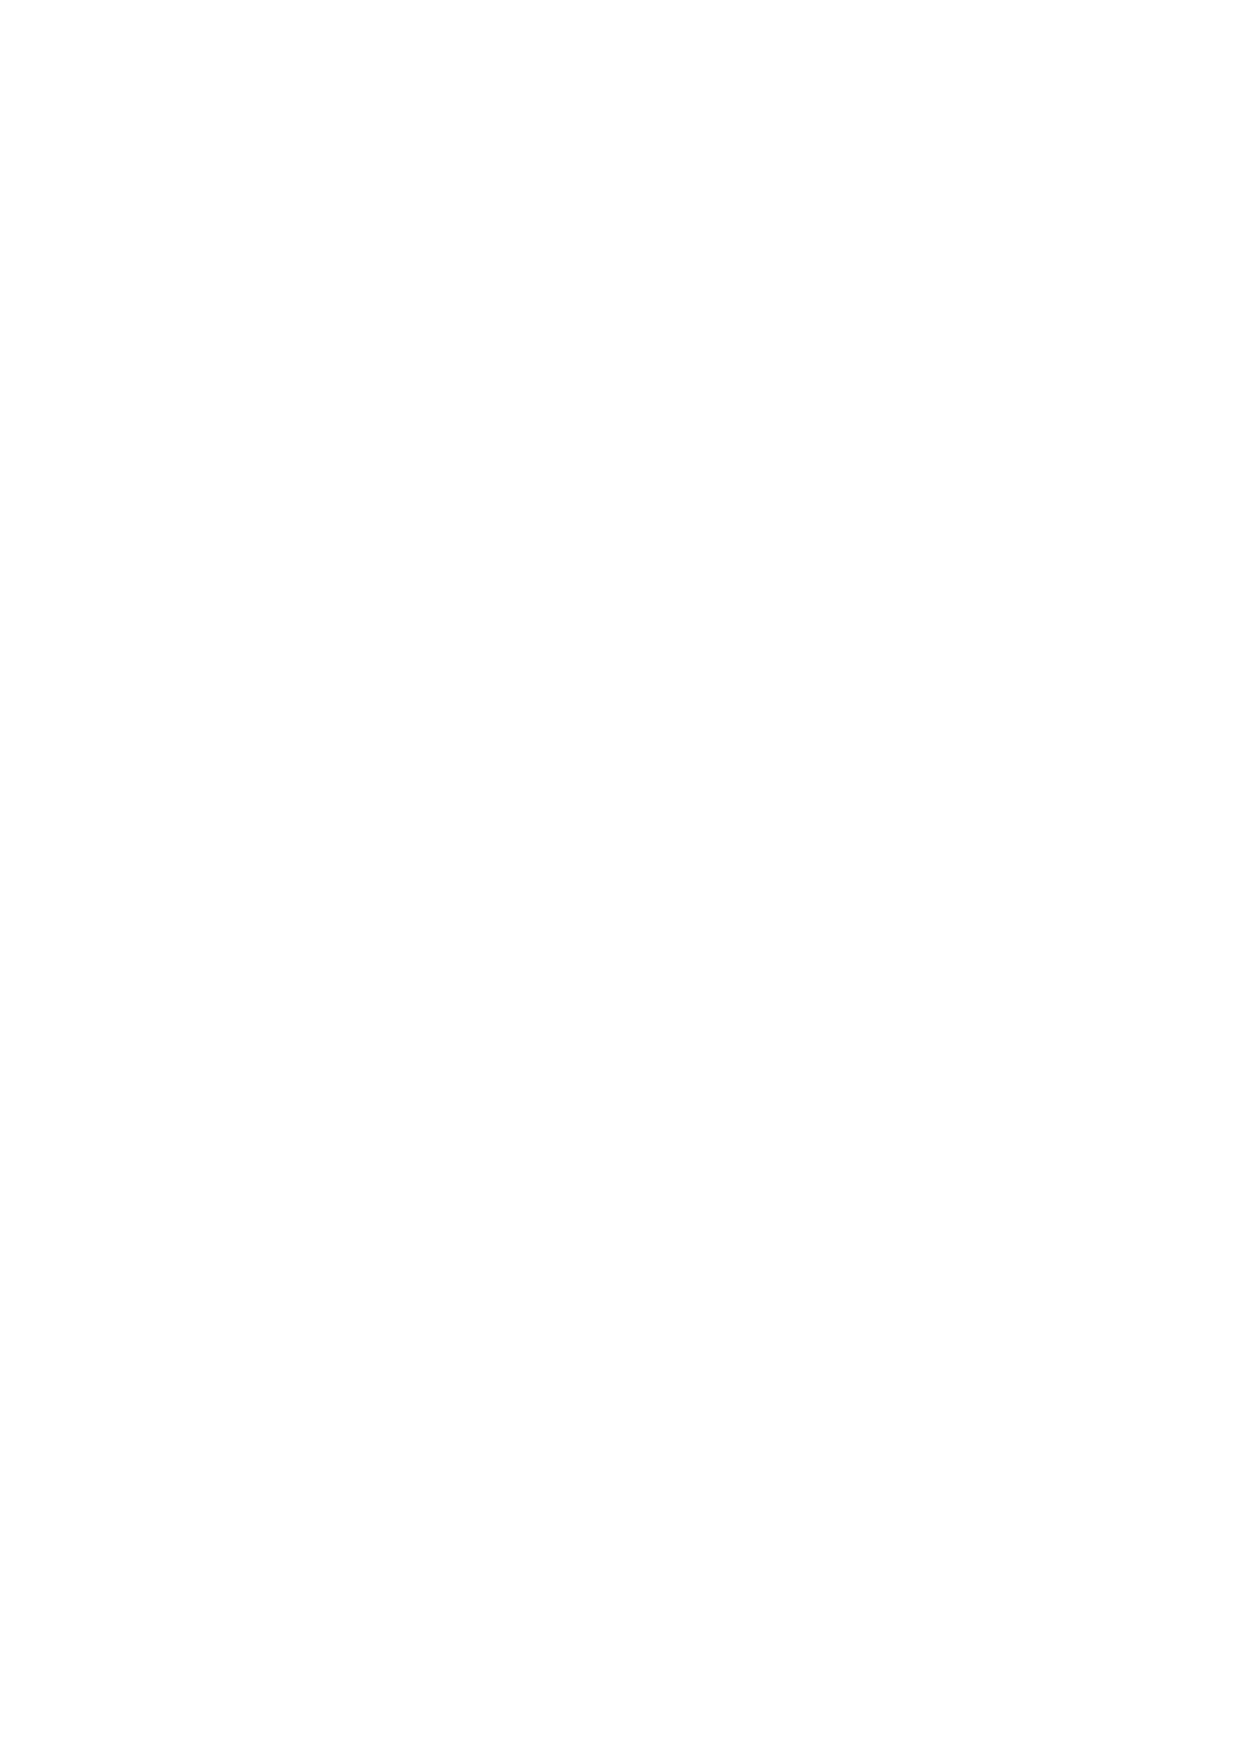
\includegraphics[width=\textwidth]{\figs/binarysearchtree}
\end{figure}

\section{Formal definition}
\termdefinition{Binary tree}{ Binary tree is a set of 3 \emph{disjoint} subsets, the first one is the root of the tree and the other 2 subsets are either empty or they are themselves binary trees.\cite[From Data Structures Using C and C++]{DEusingCCpp}}  


%----------------------------------------------------------------------------------------
\section{Understanding different terminologies related with binary trees}
\begin{itemize}
    \item The root is located at level 0.
    \item The children of any parent node will have a level equivalent to the level of the parent plus one. 
    \item A leaf node or external node is a node that does not have any children.
    \item An internal node is a parent node with two children. 
    \item A half-leaf node is a parent node with only one child.
    \item The height of the binary tree is the level of the leaf that is at the bottom, some books have it as the level of the leafs at the bottom + one. 
    \item Two nodes are considered siblings when they are children of the same parents. 
\end{itemize}

\subsection{Example}
\begin{itemize}
    \item Root is $A$. 
    \item $C,D,F\;\&\;G$ are leaf nodes or external nodes. 
    \item $A,B\;\&\;E$ are internal nodes. 
    \item There are no half-leafs except for node $A$.
    \item The height is 3 (considering start at 0).
    \item $(B,C),(D,E)\;\&\;(F,G)$ are siblings because they have the same parent.
\end{itemize}
\begin{figure}[H]
    \centering
    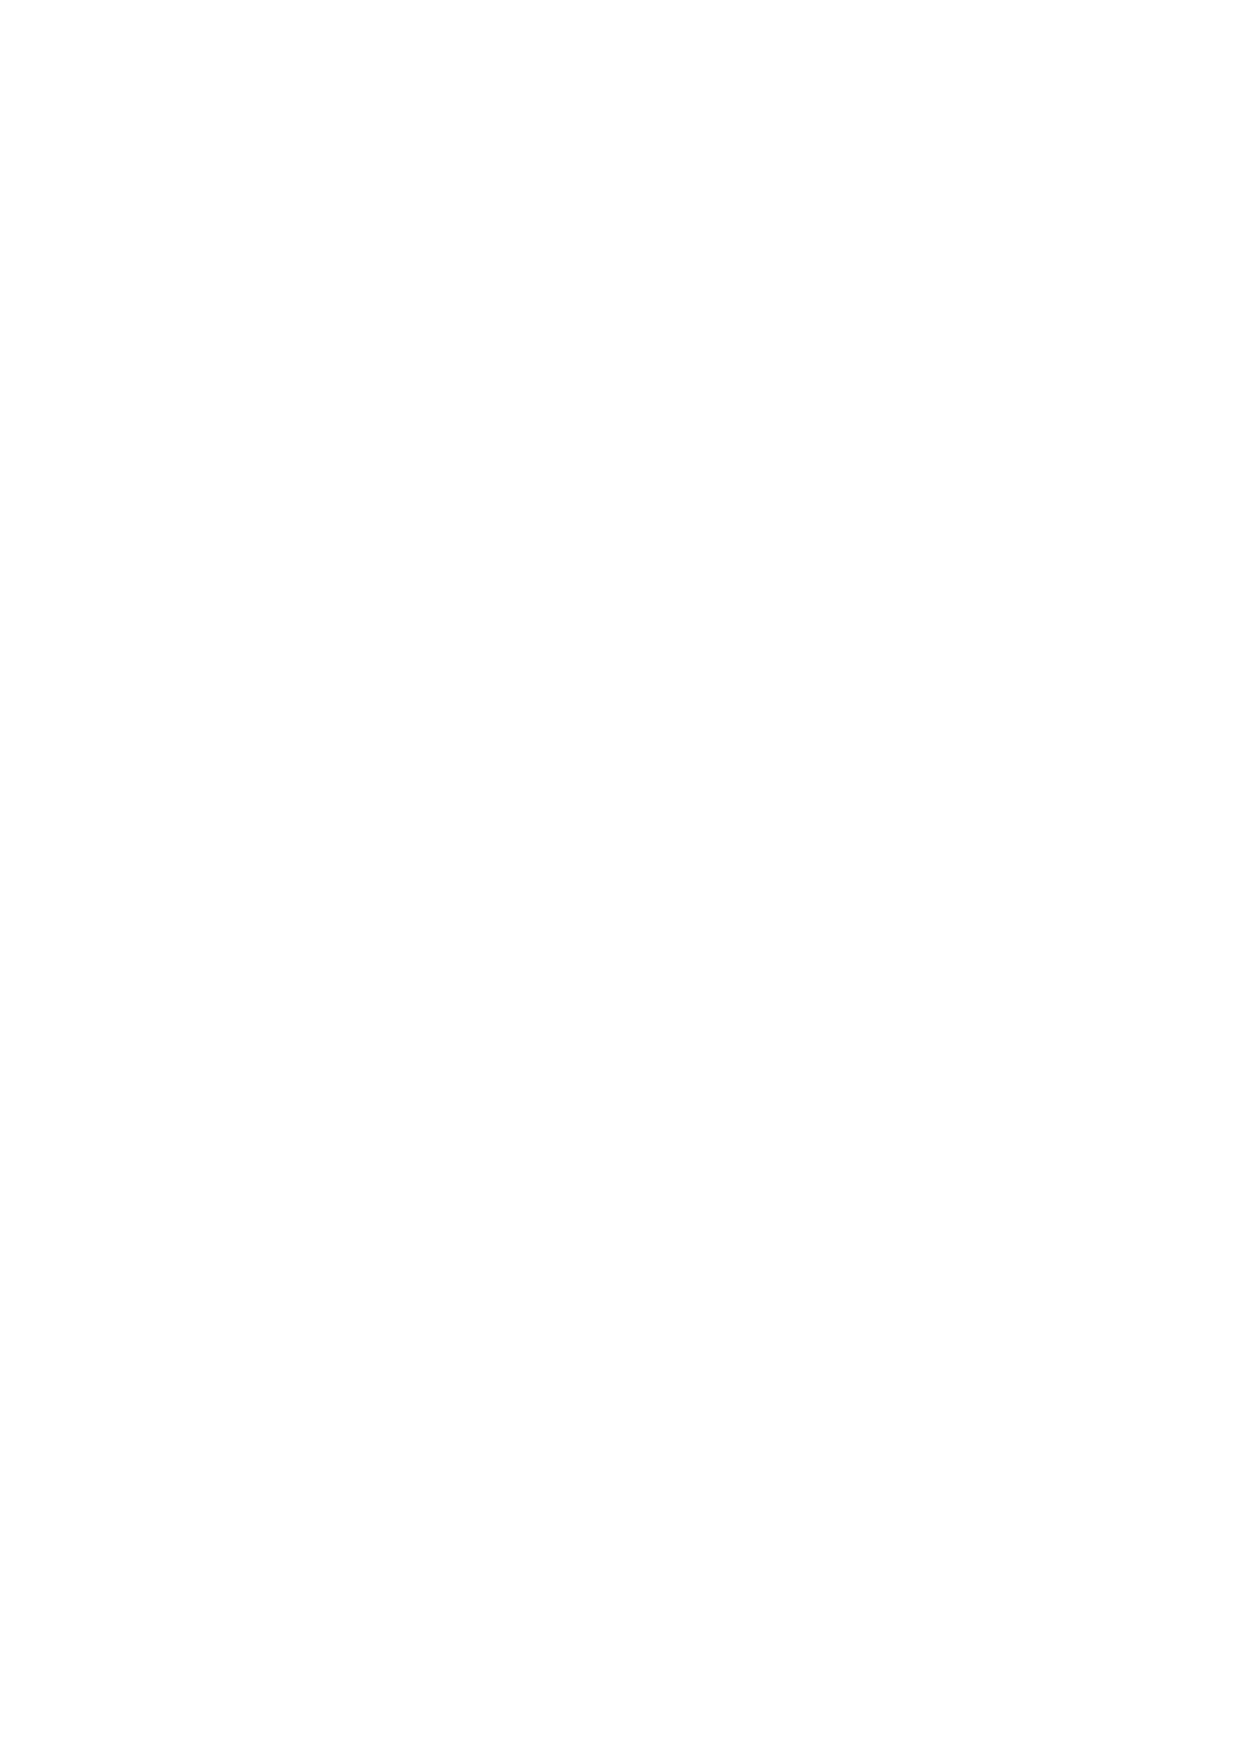
\includegraphics[width=\textwidth]{\figs/binarysearchtreeterminology}
\end{figure}

\section{Two tree / strictly binary tree}
\begin{itemize}
    \item \termdefinition{Two tree or strictly binary tree}{ is a binary tree where each node is either a leaf, or they are having both children. Meaning no half-leaf nodes.} 
\end{itemize}
\begin{figure}[H]
    \centering
    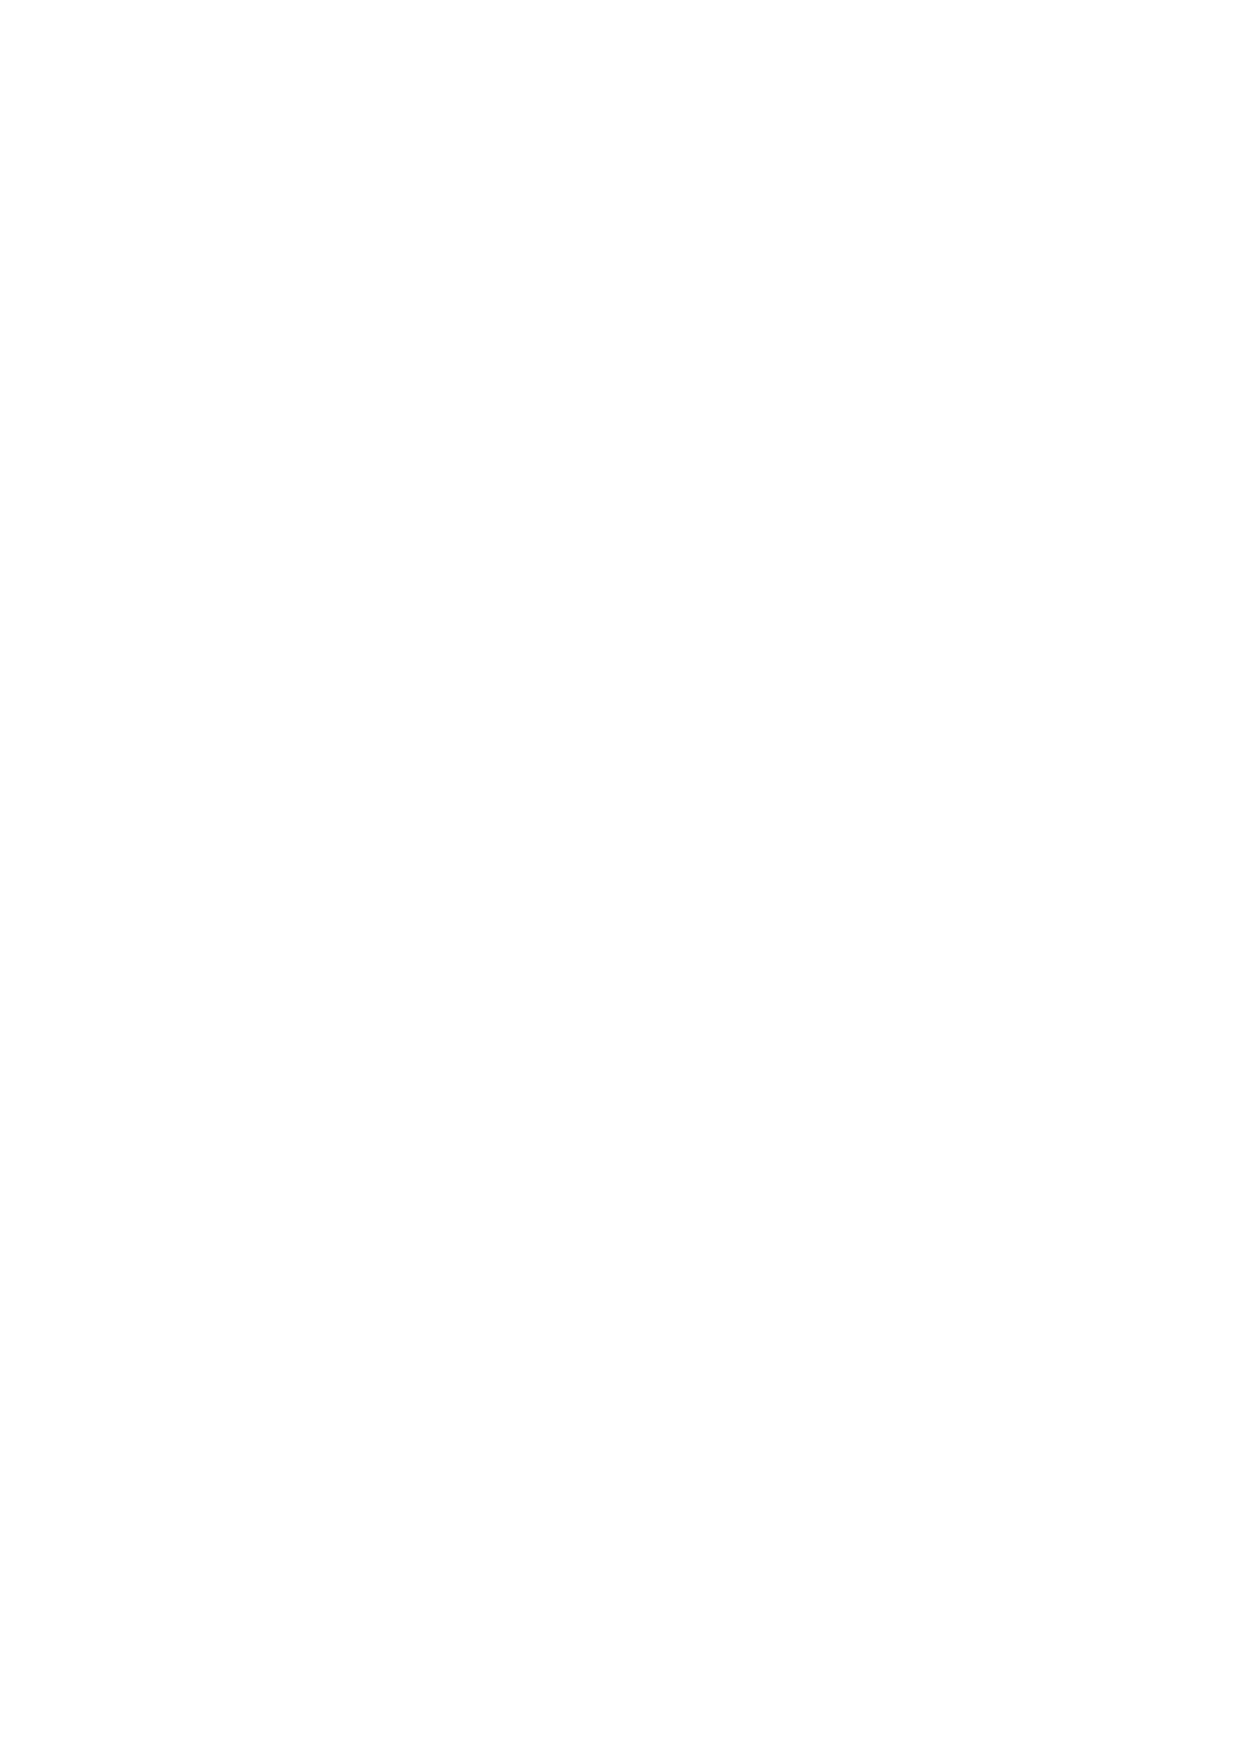
\includegraphics[width=\textwidth]{\figs/strictlybt}
\end{figure}

\section{Complete binary tree / full tree}
\begin{itemize}
    \item \termdefinition{Complete binary tree / full tree }{ A complete binary tree is a 2-tree where all leaves must reside at the same level. OR, in a complete binary tree at any leaf $k$, there are always $2k$ nodes.}
\end{itemize}
\begin{figure}[H]
    \centering
    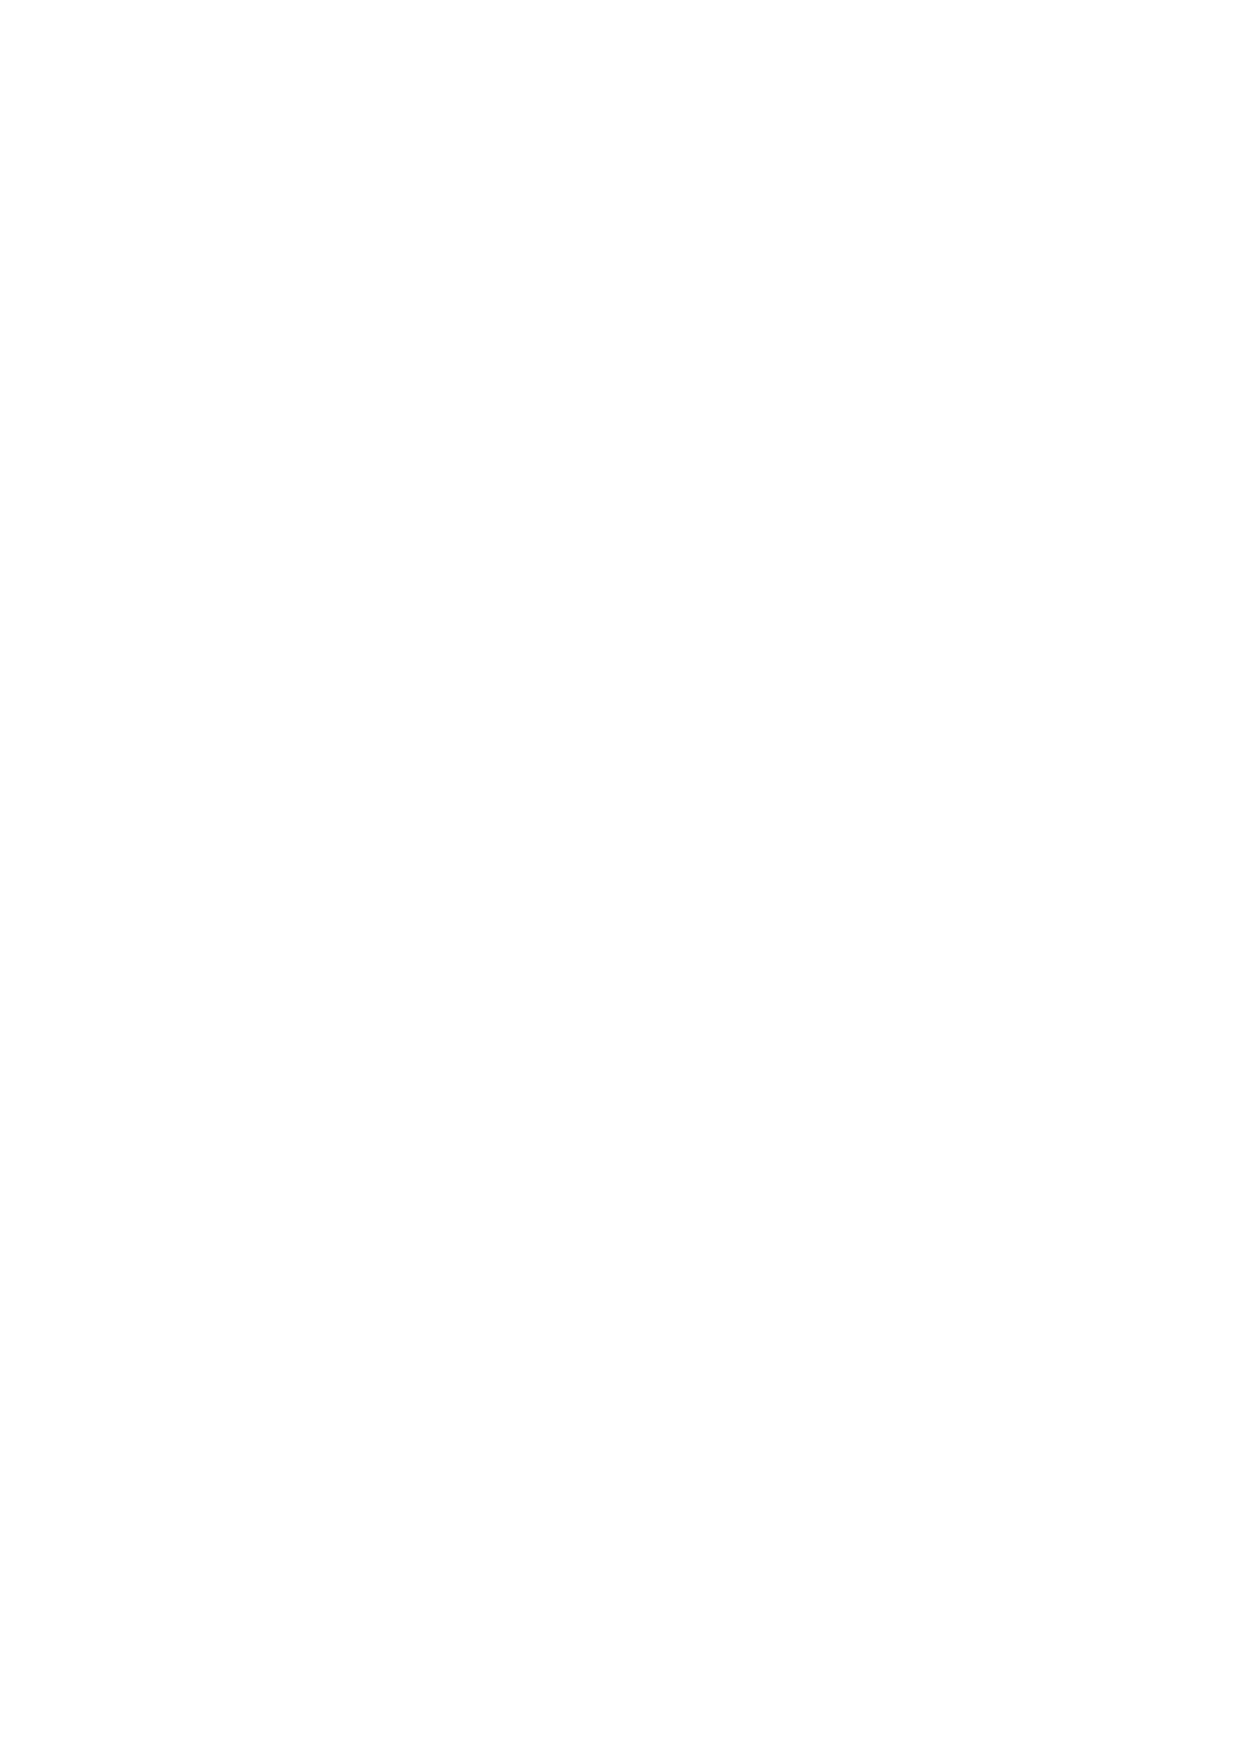
\includegraphics[width=\textwidth]{\figs/completebt}
\end{figure}
\begin{itemize}
    \item The total nodes in a complete binary tree is calculated by: 
        \[
          t_n = 2^{h+1}-1
        \]
        or \[
          t_n = 2^0+2^1+2^2+2^3+\dots+2^h
        \]
        Where the $h$ is the height.
        \begin{itemize}
            \item In the example above is $2^{2+1}-1 = 8-1 = 7$.
        \end{itemize}
    \item To calculate the number of non-leaves.
        \[
          \text{ non-leaves } = 2^h-1
        \]
    
    \item Total leaves: 
        \[
          \text{ total-leaves }=2^h
        \]
\end{itemize}


%----------------------------------------------------------------------------------------
\section{How to traverse a binary tree}
There are three strategies for traversing a binary tree:
\begin{enumerate}
    \item In-order traversal.
    \item Pre-order traversal.
    \item Post-order traversal.
\end{enumerate}
In a binary trees it's impossible to traverse linearly, they are not like arrays or linked lists in the sense where you can do a loop and traverse. Trees are not linear data structures and in order to visit every node of the tree at least once we need to have proper traversal strategies. Whenever we traverse a binary tree we must do it recursively. 

\subsection{In-order traversal strategy}
This strategy consists of implementing a recursive algorithm. This algorithm considers every current node as a sub-tree in itself.
\begin{enumerate}
    \item Traverse the left sub-tree using in-order routine. 
    \item Access root.
    \item Traverse right sub-tree using in order routine.
\end{enumerate}
\begin{figure}[H]
    \centering
    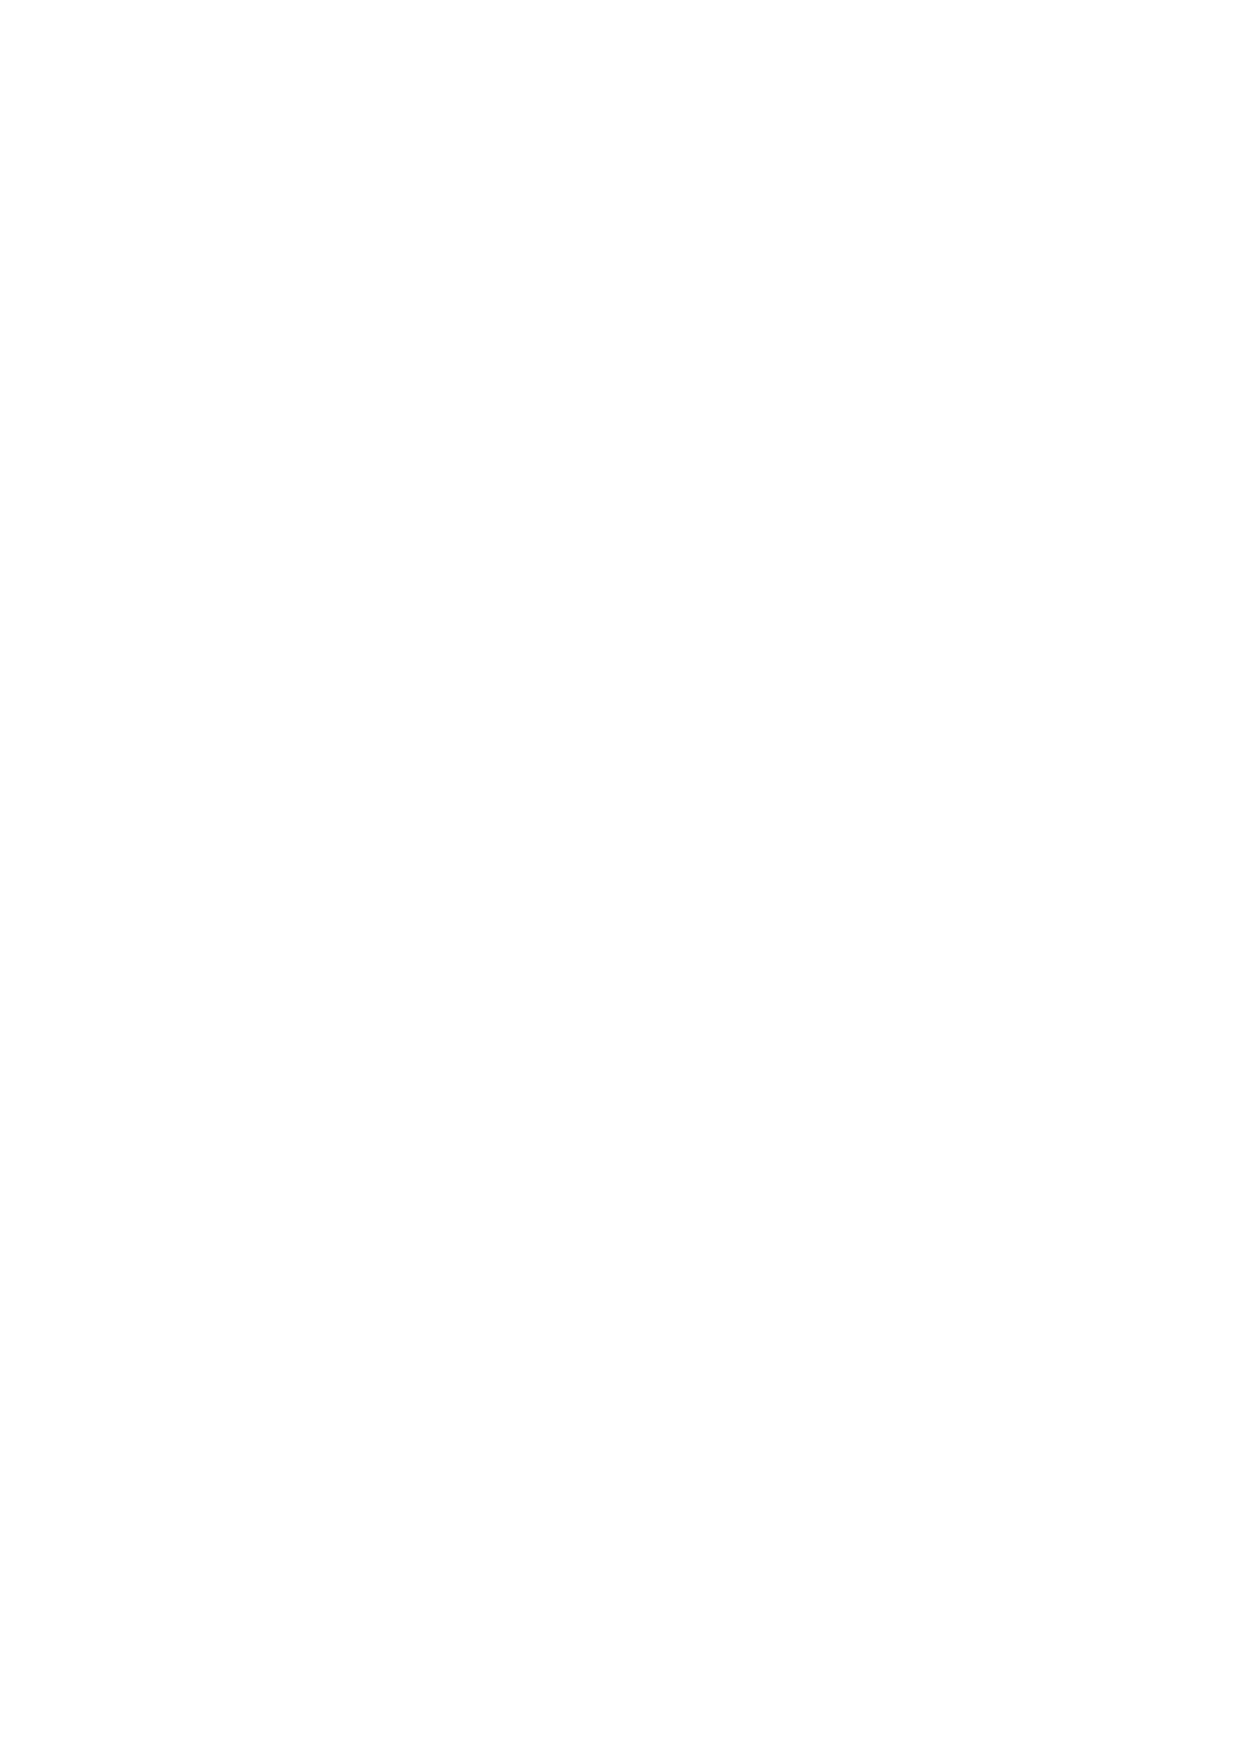
\includegraphics[scale=1.1]{\figs/inordertraversal}
\end{figure}


%----------------------------------------------------------------------------------------
\subsection{Pre-order traversal strategy}
It's different from the in-order because here the root stays constant, this algorithm doesn't consider each node the root.
\begin{enumerate}
    \item Access the root. 
    \item Traverse left sub-tree using the pre-order algorithm using recursion. 
    \item Traverse right-sub-tree using pre-order.
\end{enumerate}
\begin{figure}[H]
    \centering
    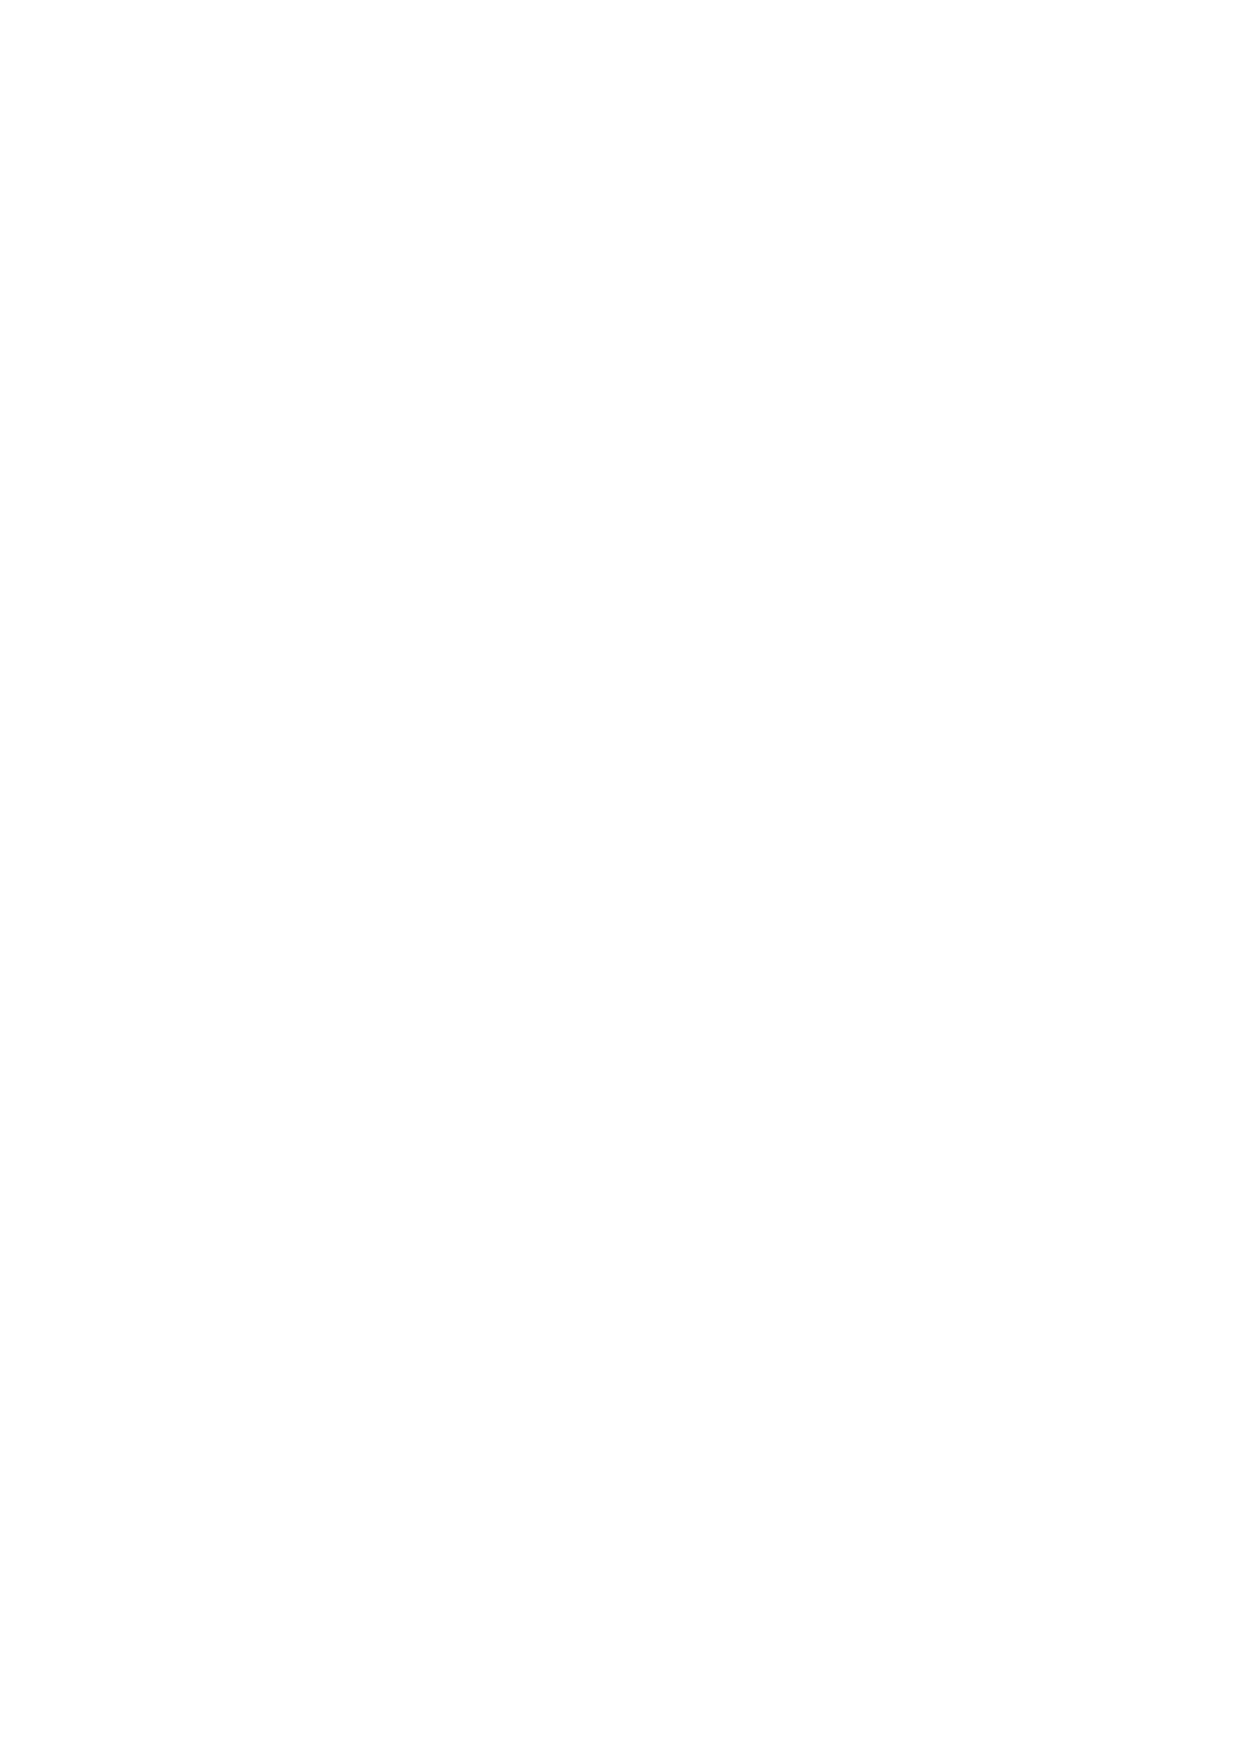
\includegraphics[scale=1.1]{\figs/preorderbt}
\end{figure}


%----------------------------------------------------------------------------------------
\subsection{Post-order traversal strategy}
In this implementation the root is accessed at the end. The position where we access the root is at the end. This is also recursive. 
\begin{enumerate}
    \item Traverse the left-sub-tree using post-order. 
    \item Traverse the right-sub-tree using post-order.
    \item Access the root.
\end{enumerate}
\begin{figure}[H]
    \centering
    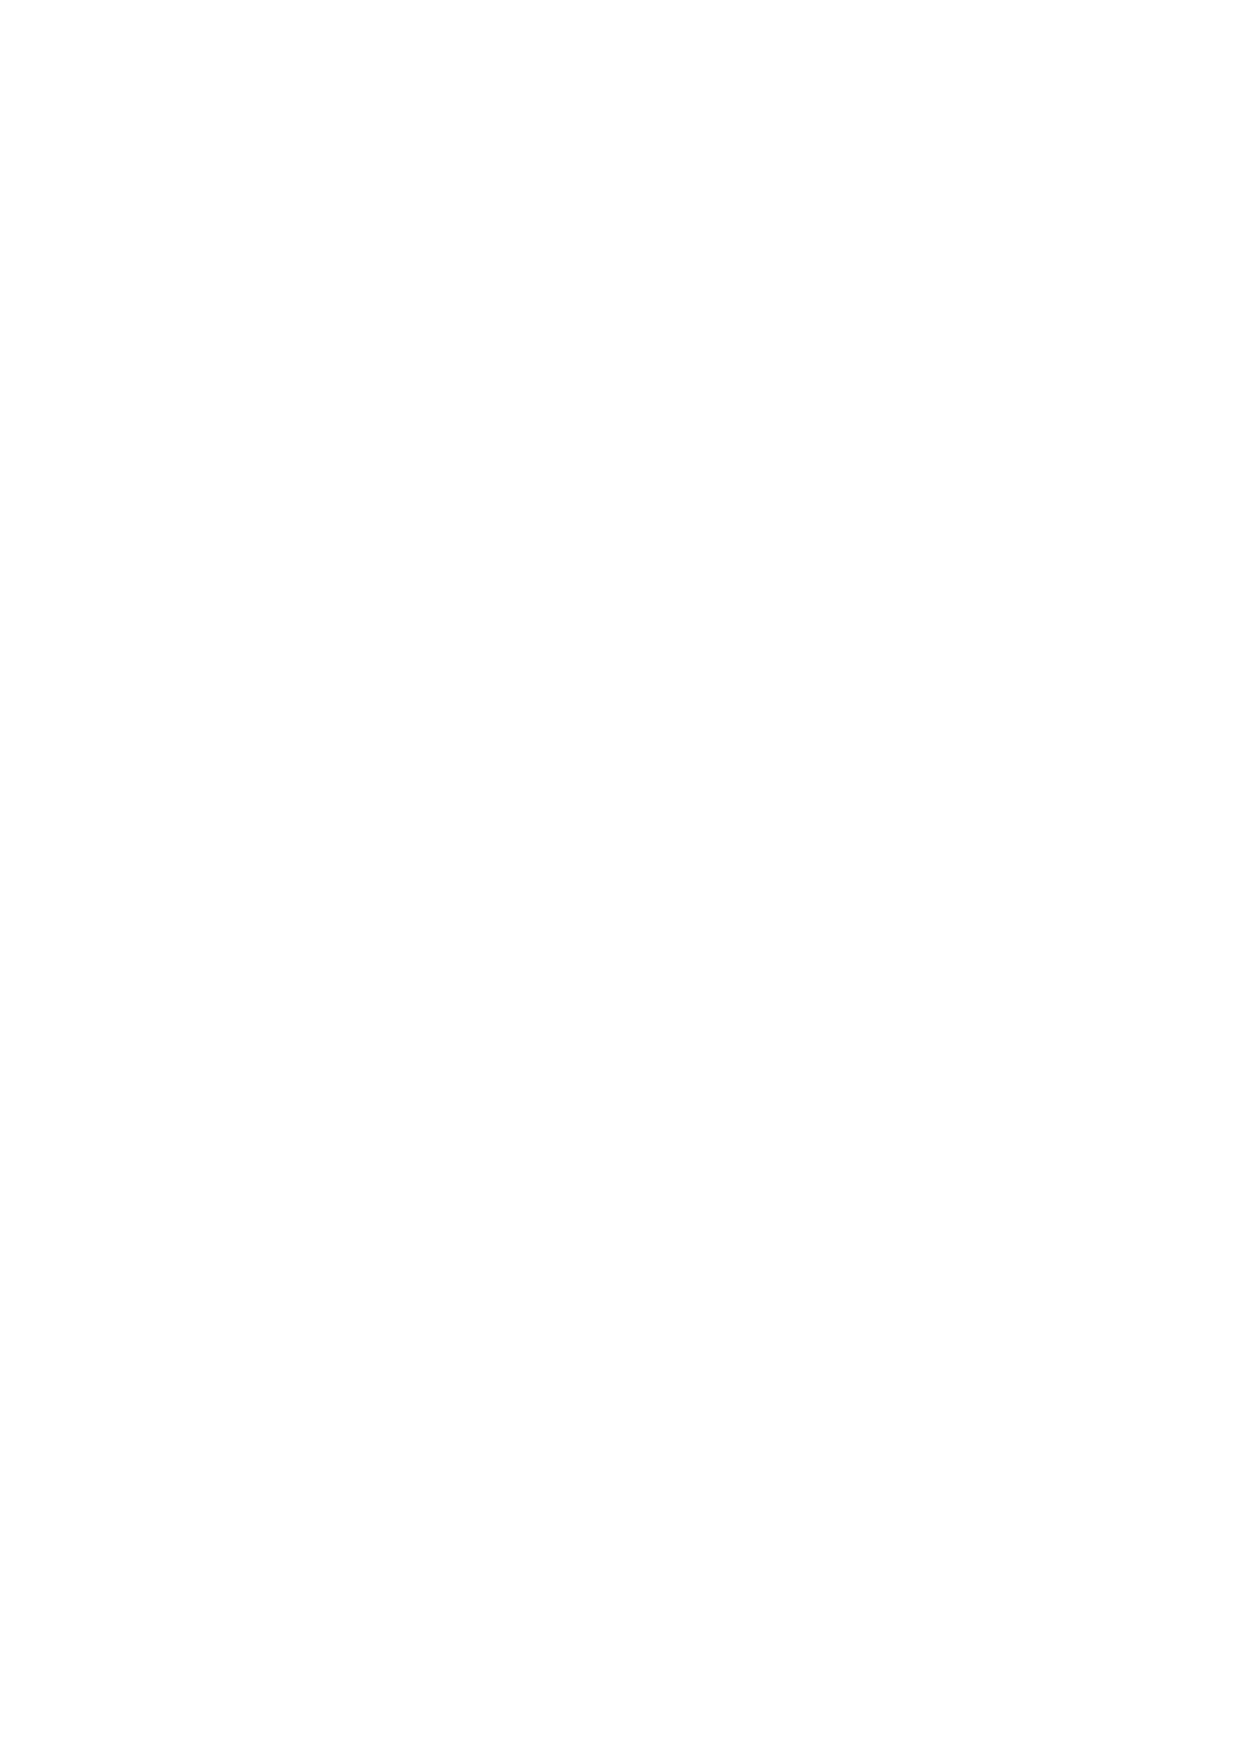
\includegraphics[scale=1.1]{\figs/postorderbt}
\end{figure}


%----------------------------------------------------------------------------------------
\section{Constructing a binary tree from a given traversal list}
\begin{itemize}
    \item In-order traversal list: $D,B,F,E,G,A,H,C,I$
    \item Pre-order traversal list: $A,B,D,E,F,G,C,H,I$
    \item Post-order traversal list: $D,F,G,E,B,H,I,C,A$
\end{itemize}

\subsection{Developing the tree using the in-order and pre-order lists}
\begin{itemize}
    \item The pre-order traversal, we access the root of the entire tree first. Thus, $A$ will be the root of the tree.
    \item In the in-order traversal, we locate $A$, we know that everything to the left of A in the in-order traversal list is the left sub-tree and everything to the right is the right sub-tree.
        \begin{itemize}
            \item With this information we know that: 
            \begin{figure}[H]
                \centering
                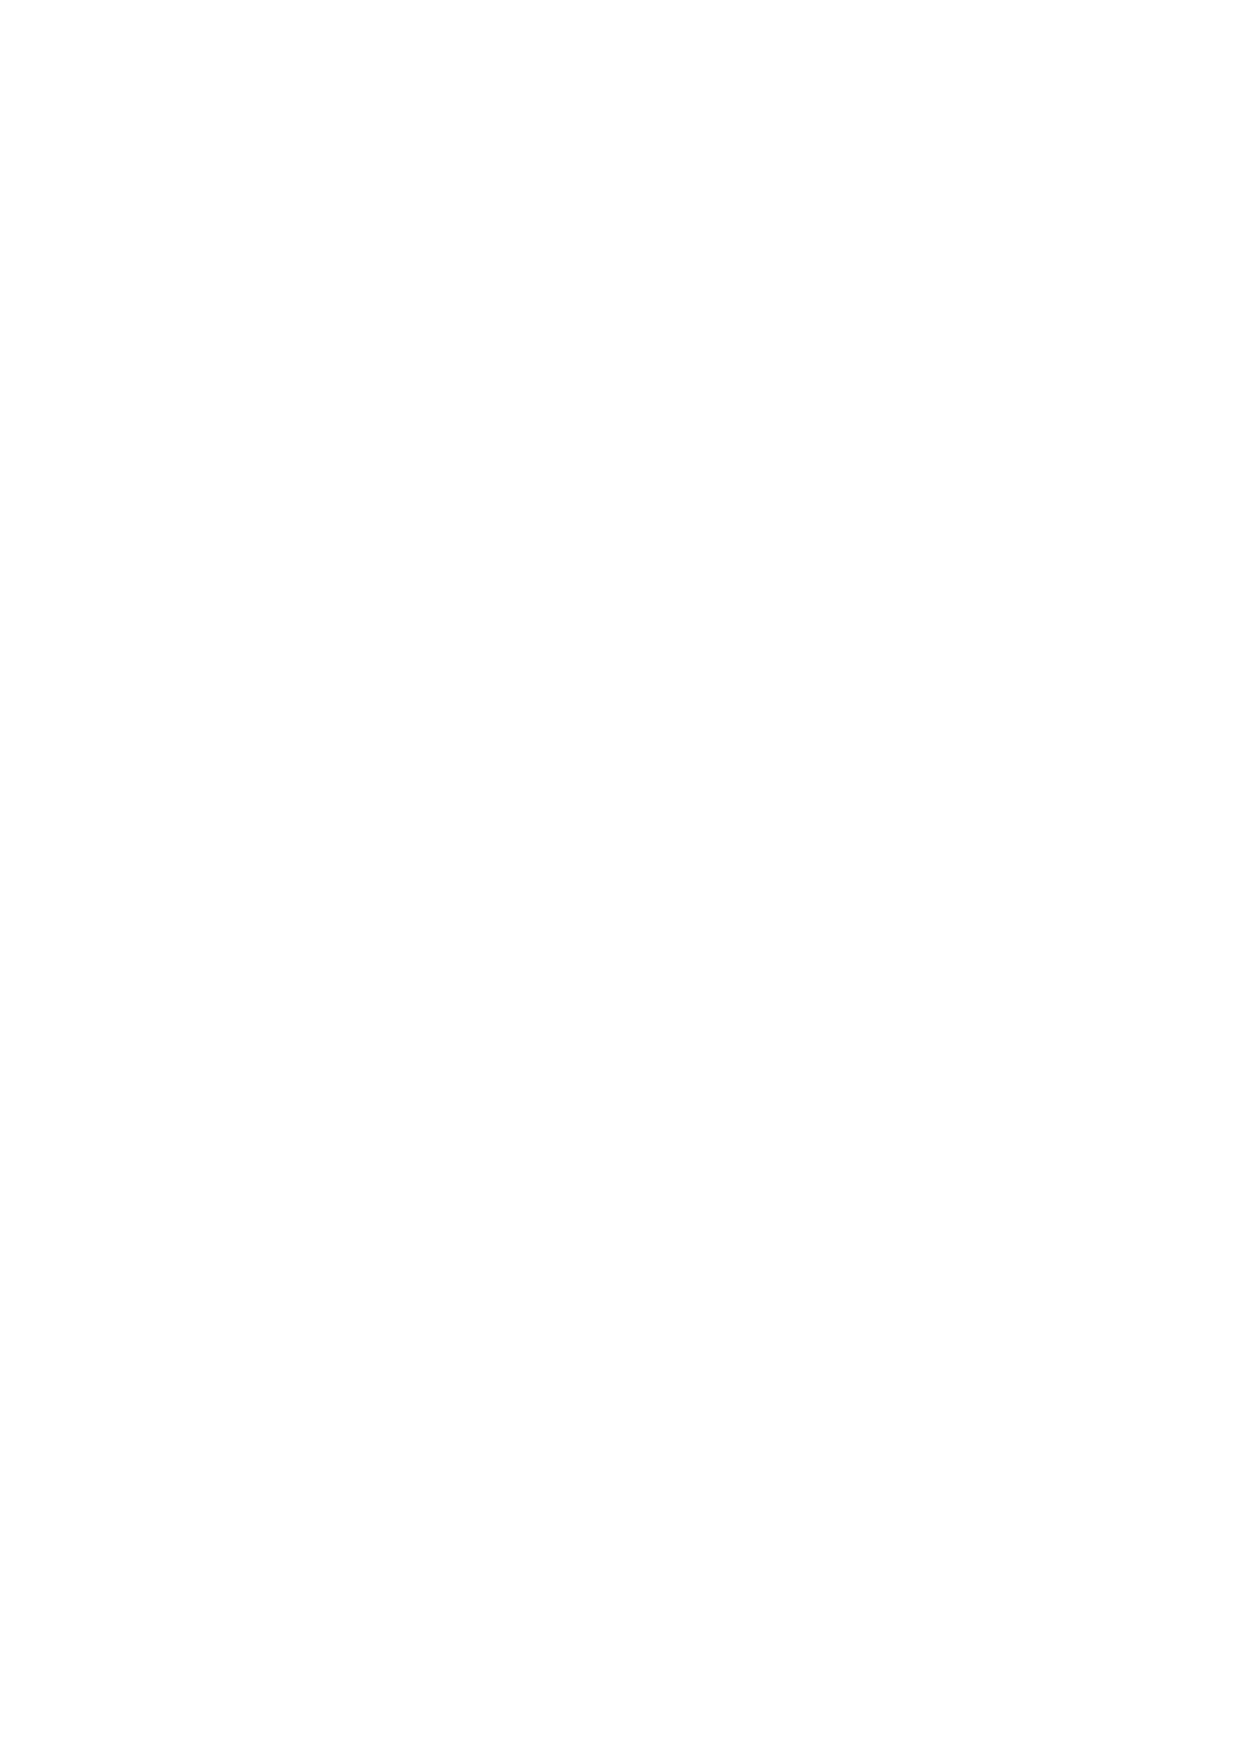
\includegraphics[]{\figs/constructingbt}
            \end{figure}
        \end{itemize}

    \item Know exmining the elements of the left subtree, we have $D,B,F,E,G$ Notice that these elements exist consecutively after the A in the pre-order traversal, not ordered but consecutively:
        \[
            \text{ Pre-order traversal list: }\; A,\overbrace{B,D,E,F,G}^{\text{ L. sub-tree }},C,H,I 
        \]
    
    \item By examining the rest, this means the remaining letters: $C,H,I$ are the right sub-tree.
        \[
            \text{ Pre-order traversal list: }\; A,B,D,E,F,G,\overbrace{C,H,I}^{\text{ R. sub-tree }} 
        \]
    
    \item Notice in the pre-order traversal, the first letter of the left sub-tree is $B$, this means the $B$ is the root of the left sub-tree.
    \item Now, locate $B$ in the in-order traversal list, anything to the left of $B$ is the left sub-tree of root $B$ and anything to the right is the right sub-tree of root $B$.
        \begin{align*}
            \text{ Pre-order traversal list of the L. sub-tree of root B:}\quad & B,D,E,F,G \\
            \text{ In-order traversal list of the L. sub-tree of root B: }\quad & \overbrace{D}^{\text{ R.sub-tree }},B,\overbrace{F,E,G}^{\text{ L. sub-tree }} \\
        \end{align*}
    
    \item Notice in the pre-order traversal, the first letter of the right sub-tree is $C$, thus this is the root of the right sub-tree.
    \item Now, locate $C$ in the in-order traversal list, anything to the left is the left sub-tree, anything to the right is the right sub-tree.
    
    \item With the information thus discovered we know the following: 
        \begin{align*}
            \text{ Pre-order traversal list of the R. sub-tree of root C:}\quad & \overbrace{C}^{\text{ Root }},H,I \\
            \text{ In-order traversal list of the R. sub-tree of root C: }\quad & \overbrace{H}^{\text{ L. sub-tree }},C,\overbrace{I}^{R. sub-tree} \\
        \end{align*}
        \begin{figure}[H]
            \centering
            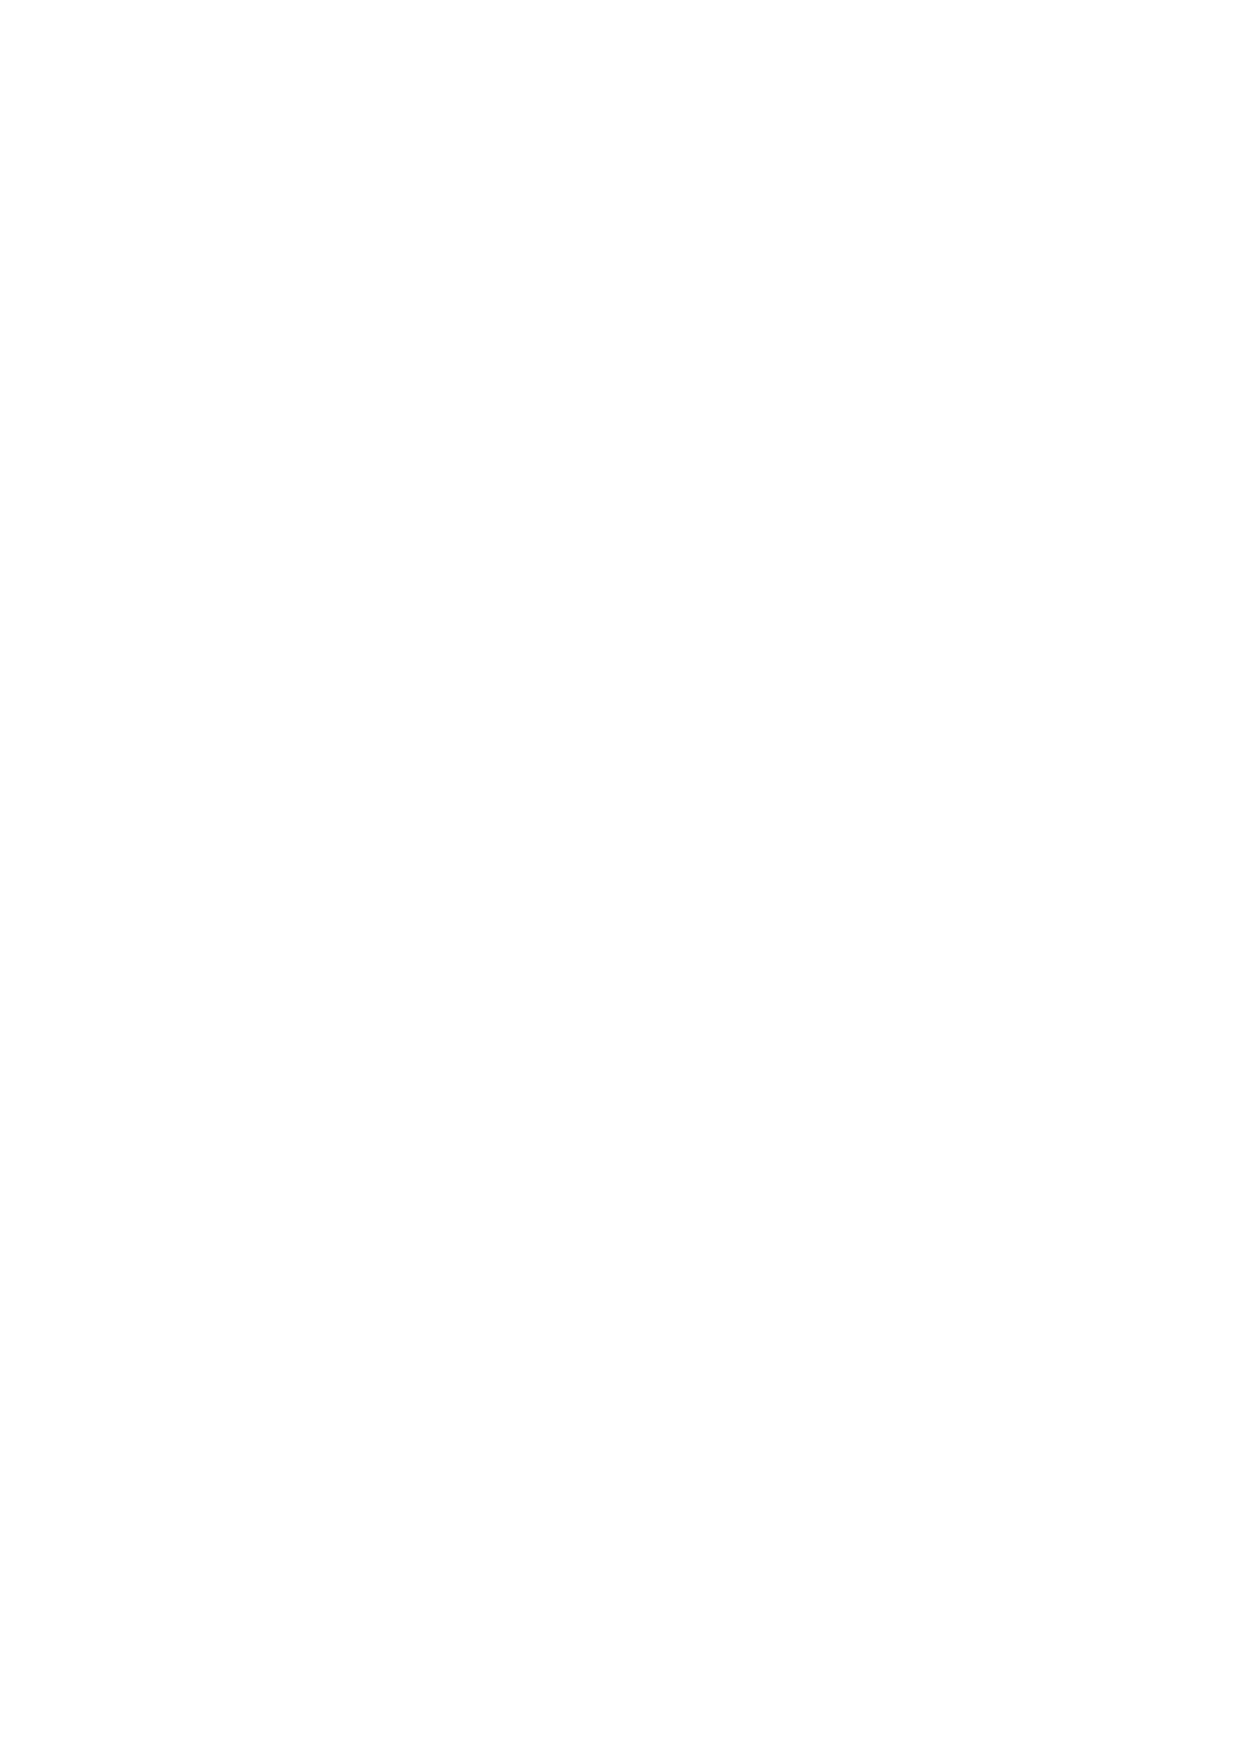
\includegraphics[]{\figs/constructingbt1}
        \end{figure}
    
    \item Notice the pre-order traversal $A,B,D,E,F,G,C,H,I$ after the $D$ the next is the $E$ this means this is the root of the right sub-tree of the tree of root $B$. 
    \item Notice with the in-order traversal list corresponding to the right sub-tree of tree of root $B$: $F,E,G$, $E$ is the root, this means anything to the left is the left sub-tree, anything to the right is the right sub-tree of tree root $E$. 
    \item Repeat the process for the $C$ right sub-tree.
    \item The end result is:
        \begin{figure}[H]
            \centering
            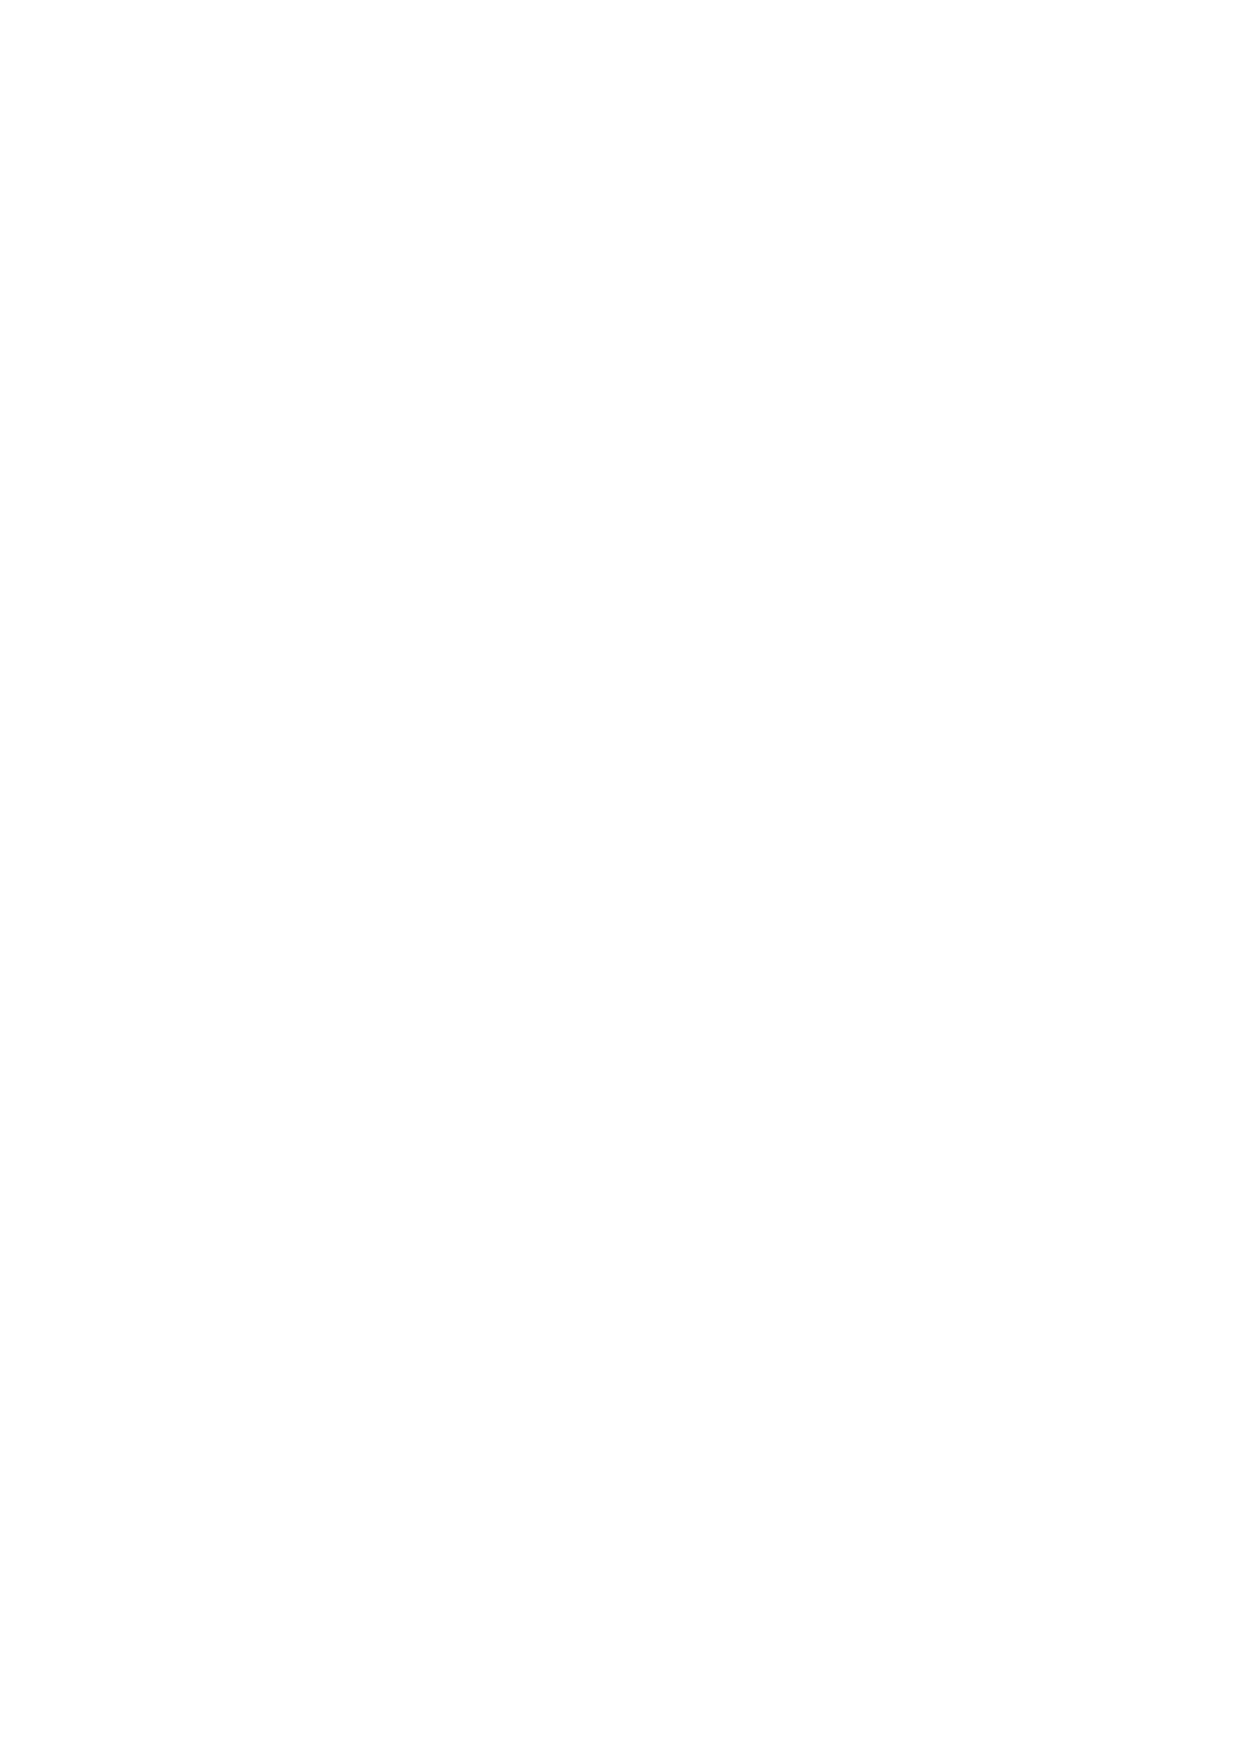
\includegraphics[]{\figs/constructingbt2}
        \end{figure}
\end{itemize}

\subsection{Developing a tree from in-order and post-order traversal lists}
% \item In-order traversal list: $D,B,F,E,G,A,H,C,I$
% \item Pre-order traversal list: $A,B,D,E,F,G,C,H,I$
% \item Post-order traversal list: $D,F,G,E,B,H,I,C,A$
\begin{itemize}
    \item The root of the tree is the very last element, in this case it's $A$ .
    \item Track $A$ in in-order traversal. Left: $D,B,F,E,G,$ Right: $H,C,I$.
    \item Identify the left and right tree in the in-order traversal list, then track the contents of both trees to the post order traversal list. Right: $H,I,C$ Left: $D,F,G,E,B$ read from left to right.
    \item The right sub-tree traversal list of root $A$'s  last letter is the root of the Right sub-tree. Right: $H,I,C$ so $C$ is the root of the right sub-tree. Checking in the in-order traversal list we find the root $C$, anything to the left is the left sub-tree, and the same for the right. In-order traversal: $H,C,I$, $H$ is the left sub-tree and $I$ is the right-sub-tree. 
    \item The left sub-tree traversal list of root $A$'s last letter is the root of the left sub-tree. Left: $D,F,G,E,B$ so root is $B$. Checking them in the in-order traversal list we find the root $B$ in $D,B,F,E,G$ to the left we have the left sub-tree, same for the right. 
    \item Repeating the process should land us in the same result. 
\end{itemize}

\section{How to define a structure of a Node for a binary tree}
We need three elements:
\begin{enumerate}
    \item A search key: 
    \item Left-pointer: pointing to the left sub-tree, if no sub-tree point to null. 
    \item Right-pointer: pointing to the right sub-tree, if no sub-tree point to null.
\end{enumerate}

\section{Binary search tree}
\begin{itemize}
    \item To apply binary search on list/array elements, the list or array must be sorted.
    \item Sorting algorithms worse case complexity of quicksort or merge sort is $O(n*\log_{}\p{ n } )$.
    \item The worse case complexity of binary search is $O(\log_{}\p{ n } )$.
    \item The overall instead of sorting with quick sort or merge sort and getting complexity $O(n*\log_{}\p{ n } )$ performance, using a binary search tree the elements will be accomodated while they are being inserted thus the complexity will always be $O(\log_{}\p{ n } )$.
\end{itemize}
Binary search tree definition: 
\begin{figure}[H]
    \centering
    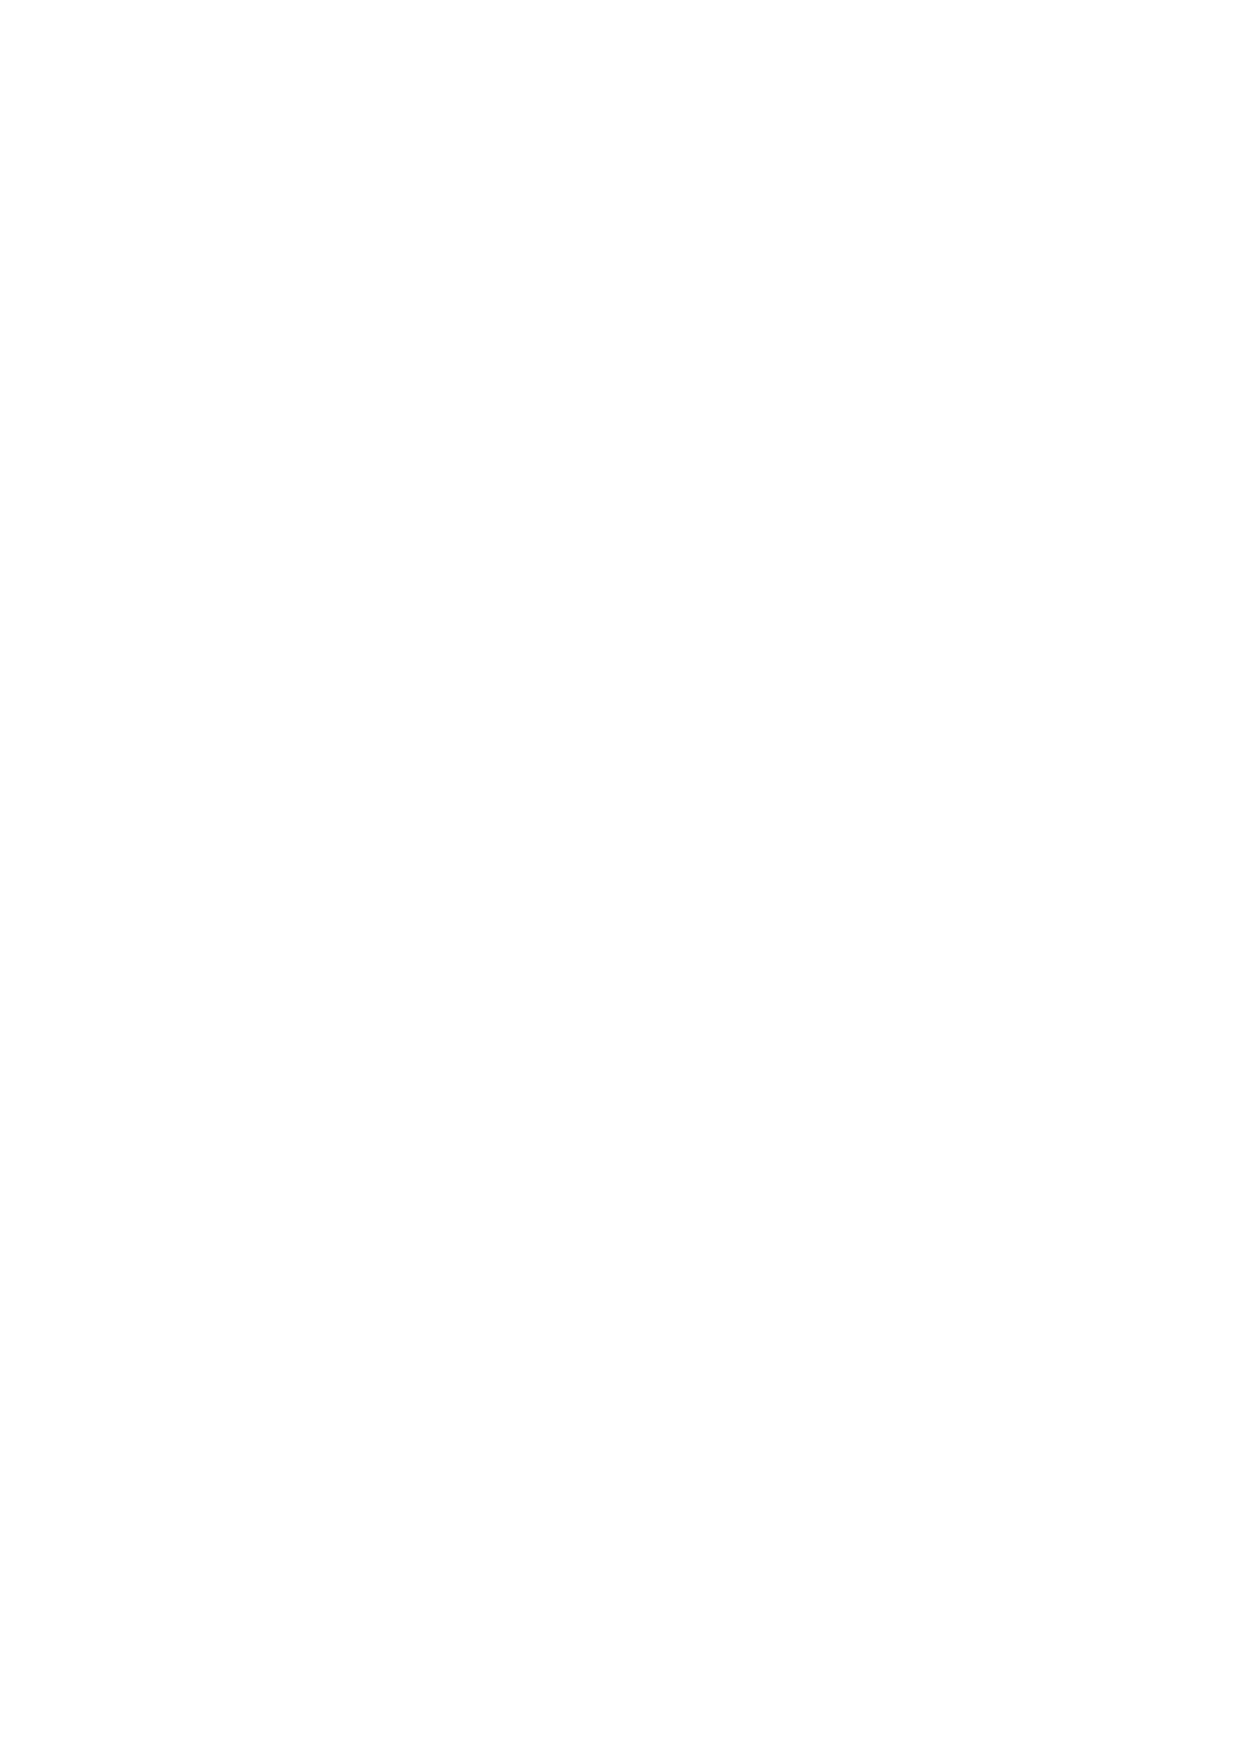
\includegraphics[]{\figs/binary_search_tree}
\end{figure}
Example: 
\begin{figure}[H]
    \centering
    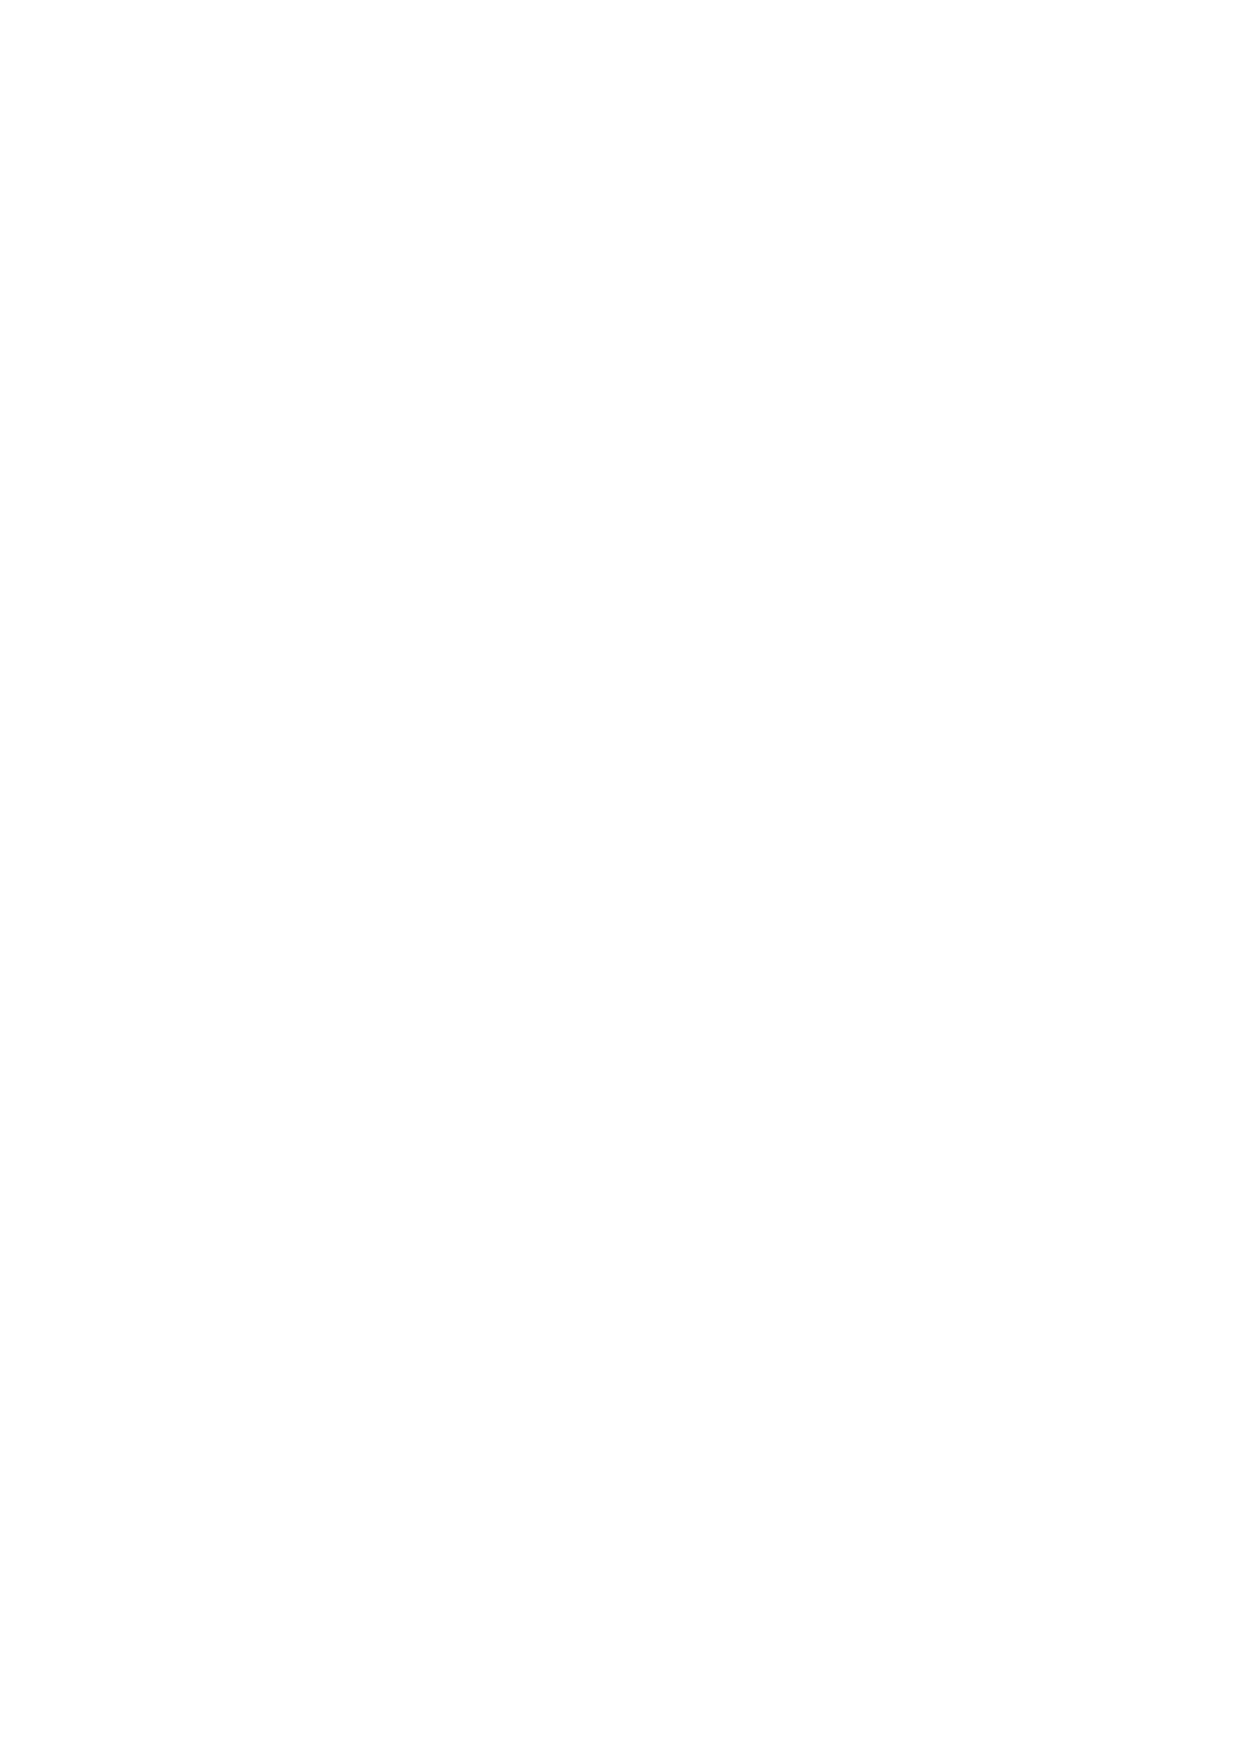
\includegraphics[]{\figs/binary_search_tree_example}
\end{figure}

\section{Binary tree implementation}
\inputcode{c}{\code/binary_tree.c}
